% Metódy inžinierskej práce

\documentclass[10pt,oneside,english,a4paper]{article}

\usepackage[english]{babel}
%\usepackage[T1]{fontenc}
\usepackage[IL2]{fontenc} % lepšia sadzba písmena Ľ než v T1
\usepackage[utf8]{inputenc}
\usepackage{graphicx}
\usepackage{url} % príkaz \url na formátovanie URL
\usepackage{hyperref} % odkazy v texte budú aktívne (pri niektorých triedach dokumentov spôsobuje posun textu)
%\usepackage[nottoc]{tocbibind}
\usepackage{cite}
\usepackage{times}
%\usepackage{fancyhdr}

\pagestyle{myheadings}

\title{Digital revolution in learning\thanks{Semestrálny projekt v predmete Metódy inžinierskej práce, ak. rok 2020/21, vedenie: Ing. Fedor Lehocki, PhD.}} % meno a priezvisko vyučujúceho na cvičeniach

\author{Adrian Szacsko\\[2pt]
	{\small Slovenská technická univerzita v Bratislave}\\
	{\small Fakulta informatiky a informačných technológií}\\
	{\small \texttt{xszacsko@stuba.sk}}
	}

\date{\small 14. October 2020} % upravte



\begin{document}

\maketitle

\begin{abstract}
Nowadays technology surrounds us so much, that the way we study is highly impacted
by it. We are taking advantage of the web and many of us prefer to learn new things by
searching the Google rather than using books.

	In this paper we would like to sharpen the focus to the new ways of learning as well as
self-learning, compare today’s schools to the 20. century’s educational systems, ways we
implement the newest technological advancements to help us study and the future of
learning. In the last 10 years schools and colleges started to adapt and rely more on the use
of computers and the access to the internet. We would like to point out the differences, pros
and cons of digitalization along with the traditional methods of education. 

There are many benefits of using computers in the classrooms, like maximizing student’s engagement. However, this type of
study has negative phenomenon, because computers can be distracting for the students.
Chats, video games and the internet can easily take them off task. The pandemic we face
accelerated this digital revolution by requiring computers to work and study as well.
\end{abstract}



\section{Introduction}

	Learning and the ways humanity learn is always changing. This article shows, how the technological advancements in various fields innovate learning and our school systems. Technology tries to ease the study~\ref{self-learning} to become more interesting and exciting. This article shows the comparisons between traditional and digital teaching~\ref{comparison}, the use of teaching methods and the strenghts of implementing the digitalization. We try to focus on the online teaching during this pandemic situation~\ref{covid} and the future of teaching systems~\ref{future}.



\section{Learning in new ways and self-learning}\label{self-learning}

	Innovations which nowadays happen in a yearly basis  help the technological advancements in many fields, including the new approaches students can learn. Part of technology education, videogames and similar applications emerged as a popular topic
in education today\cite{Okur2017}. These applications help in teaching different languages, mainly English, however students can gain other non-language skill in field like history, science, architecture or math. Many games, like Assassin's Creed Unity are based on story telling from the real world. These are mainly focused on historical events, from which the player can learn important occasions while playing. Other games, like Minecraft help children to become creative while walking around the block based open world. 

\subsection{Collective Intelligence}

	With the use of technology, students are already able to learn in different ways, however the style of tests and exams were the same throughout many decades. The term Collective Intelligence tries to change this aspect of the schooling systems. With the use of databases, teachers are able to show the data banks for a given subject and the students can learn the answers for those questions. Thanks to this method, students have a higher chance to get better marks, the stress factor is minimalized and students can  get to know, which aspects of the subject they need to improve on. The term Collective Intelligence gives a look to the database for students, teachers and even outsiders as well\footnote{This subsection of the article was created about the 9th presentation of the semester in the subject MIP by Ján Lang: Content engineering}.

\section{Comparison between traditional and digital teaching}\label{comparison}

	Technological innovations made digital teaching possible, however traditional teaching methods are still in majority. There are different use cases for each of them in which they are superior and we would like to collect them in this section. We are going to talk about:

\begin{itemize}
\item Traditional teaching~\ref{3.1}
\item Digital teaching~\ref{3.2}
\item Use of teaching methods~\ref{3.3}
\item Strenghts of digital learning~\ref{3.4}
\end{itemize}

\subsection{Traditional teaching}\label{3.1}

	The above mentioned teaching method is realized mainly in classrooms with "lecture". It refers to instructors delivering teaching matherials in the teaching activity, so called lessons, to learners to interpretation. It has been broadly used for the last couple of centuries and is still one of favorable teaching methods of instructors.\cite{Lin2017}

\subsection{Digital teaching}\label{3.2}

	This type of teaching method can be realized through classrooms with lectures, however with digitalized materials and the use of the internet or modern technologies it has the flexibility to make the lesson distant. Digital learning become the most rapidly developed learning method in the past few years and can become the mainstream in the future.\cite{Lin2017}

\subsection{Use of teaching methods}\label{3.3}

	There are various differences between teaching in traditional and digital form. These two ways of learning have their own positive and negative attributes, which highly contributes to the curiosity of the subject itself. Different material contents, learning channels, and practice methods are used between these teaching methods. Traditional teaching methods are superior for courses which require practical operations or teamwork, although learning contents focusing on convenience and flexibilty were more suitable for digital  learning. The digitalization can not replace completely traditional teaching yet, however the best teaching effect for learners are comprehensively practicing both methods in teaching activity.\cite{Lin2017}

\subsection{Strenghts of digital learning}\label{3.4}

	Digital learning has many advantages for comparison with traditional learning. This method grants learners the freedom on time and space to select the best possible date for the online course and gives no pressure on the instructor when to make the teaching activity.  \cite{Lin2017}


\section{Online teaching during the pandemic}\label{covid}

	The pandemic situation accelerated the use of technology in many institutions, including secondary schools from all over the world. According to a study\cite{Babinkov2020}, in many secondary schools across Slovakia were different experiments conducted for the students to get to know the subject easier. These experiments played a tremendous role in chemistry and science education as stated in the study, however the lockdown negatively affected these type of observations. Schools needed to transfer the theoretical and the practical aspects of the lectures to online based activities. Based on the study itself\cite{Babinkov2020}, these experiments can be introduced in the following forms:
\begin{itemize}
\item Written descriptions assisted with photos
\item Video-recorded demonstrations
\item Live interactive demonstrations
\item Live demonstrations of experiments with data logging systems
\item Simple “linear” simulations
\item Virtual laboratories in the form of advanced multithread simulations
\item Remote laboratories in the form of remote-controlled real laboratory equipment
\end{itemize}

	The online experimental methods varied from school to school, however the experiments were still made despite of the lockdown. The study shows, that teachers shared and discussed the collected data with students, contemplated the pros and cons of different experiments. According to the teachers, they convinced that this approach made lessons more interesting/attractive to students, made problems easier to understand, and gave more time for discussion of results  compared with carrying out similar experiments during regular classes. On the other hand, they regret that students did notdevelop manual laboratory skills, that multiple data sets were not explored, and that they missed the direct contact with their students, which caused, i.a., a less effective discussion \cite{Babinkov2020}.

\begin{table*}[tbh]
\centering
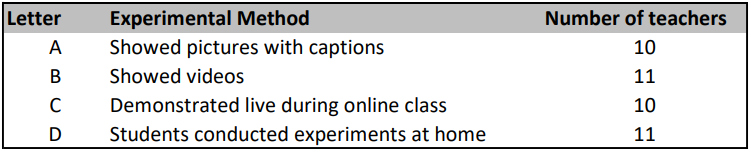
\includegraphics[scale=.6]{coronavirus_1.png}
\caption{Online Experimental Methods\cite{Babinkov2020}}
\label{f:rozhod}
\end{table*}

\begin{figure*}[tbh!]
\centering
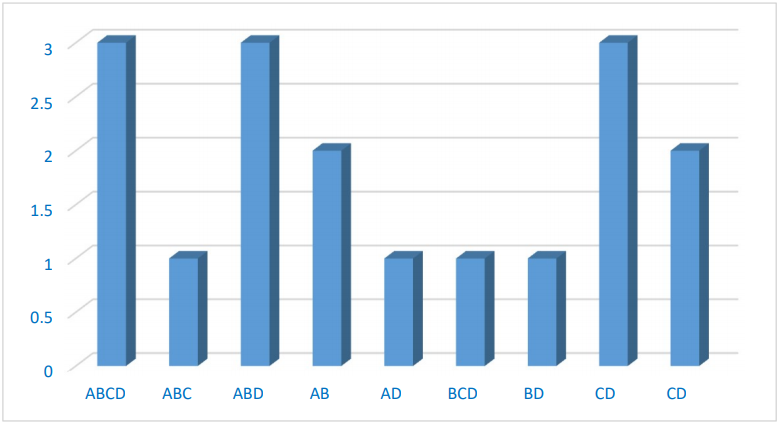
\includegraphics[scale=.55]{coronavirus_2.png}
\caption{Distribution of the sets of approaches to experiments during online chemistry lessons\cite{Babinkov2020}}
\label{f:rozhod}
\end{figure*}


\section{The future of teaching}\label{future}

	Given the pandemic, our future of teaching is starting to become reality now. Computer based equipments are helping the digitalization, however many technologies are still at science fiction level or are expensive enough to not be used in teaching enviroments. In this section, we are going to talk about:

\begin{itemize}
\item The technology itself~\ref{5.1}
\item Digital teaching~\ref{5.2}
\end{itemize}

\subsection{The technology itself}\label{5.1}

	Today's technological advancements are growing rapidly, while more and more students get surrounded by the newest gadgets. Some of them are just temporary novelties, which does not evolve into fascinating products, however there are a couple of developments which try to change the world. One of them, which can be very useful and can revolutionize the future of teaching is the augmented reality. Augmented reality is a technology, which overlays the real world with virtual objects \cite{Tretyakova2019}.


\subsection{AR technologies in teaching}\label{5.2}

	 In some fields, for instance in geometric building modeling AR has many advantages. The need naturally has arisen for teaching students new design methods at construction sites using AR technologies, i.e. creating not just a project of a building being constructed in the form of drawings, mock-ups, working documentation, but a model containing all the information about the object, which can be in demand throughout the entire period of its existence - from design, then to operation, and finally to demolition or reconstruction \cite{Tretyakova2019}. The use of AR in practice recently begun, however universities need to start to adapt this technology. 

\begin{figure*}[tbh!]
\centering

\includegraphics[scale=.6]{ar_tech.pdf}
\caption{Creation of an informational model of a building\cite{Tretyakova2019}}
\label{f:rozhod}
\end{figure*}

\section{Conclusion}

	This article shows, that technology can be used in numerous ways in schooling systems. Traditional, non-technology implemented subjects are slowly disappearing, thanks to the variety of technological advancements. The use of AR, VR and mixed reality starts to get into our lives through learning activities, however it has to be implemented in a greater extent.



%\acknowledgement{Ak niekomu chcete poďakovať\ldots}


% týmto sa generuje zoznam literatúry z obsahu súboru literatura.bib podľa toho, na čo sa v článku odkazujete
\bibliography{literatura}
\bibliographystyle{plain} % prípadne alpha, abbrv alebo hociktorý iný
\end{document}
